\begin{frame}
\frametitle{Objectives}
\begin{itemize}
\item Understand MiniZinc IDE
\item Bundled Solvers
\item Basic Modelling in MiniZinc
\item Some More Examples
\end{itemize}
\end{frame}

\begin{frame}
\frametitle{Outline}
\begin{itemize}
\item MiniZinc Background
\item IDE
\item Elements of MiniZinc Programs
\item Running Programs
\end{itemize}
\end{frame}

\section{MiniZinc Background}

\begin{frame}
  \frametitle{MiniZinc}
  \begin{itemize}
  \item Developed in the Australian NICTA project
  \item Maintained by Monash University
  \item Modelling tool with multiple back-end solvers
  \item Available from \url{https://www.minizinc.org/}
  \end{itemize}
\end{frame}

\begin{frame}
\frametitle{Framework Process}
\begin{center}
\begin{tikzpicture}[xscale=2]
\node[shape=rectangle,fill=pantone127-4] (problem) at (2.5,5) {Problem};
\node (human) at (2.5,4) {Human};
\node[shape=rectangle,fill=pantone127-4] (model) at (2.5,3) {Model};
\node (compile) at (2.5,2) {Compile/Reformulate};
\node (solver1) at (1,1) {CP};
\node (solver2) at (2,1) {MIP};
\node (solver3) at (3,1) {SAT};
\node (solver4) at (4,1) {Other};
\node[shape=rectangle,fill=pantone157-8] (solution1) at (1,0) {Solution};
\node[shape=rectangle,fill=pantone157-8] (solution2) at (2,0) {Solution};
\node[shape=rectangle,fill=pantone157-8] (solution3) at (3,0) {Solution};
\node[shape=rectangle,fill=pantone157-8] (solution4) at (4,0) {Solution};
\draw[-] (problem) -- (human);
\draw[->] (human) -- (model);
\draw[-] (model) -- (compile);
\draw[-] (compile) -- (solver1);
\draw[-] (compile) -- (solver2);
\draw[-] (compile) -- (solver3);
\draw[-] (compile) -- (solver4);
\draw[->] (solver1) -- (solution1);
\draw[->] (solver2) -- (solution2);
\draw[->] (solver3) -- (solution3);
\draw[->] (solver4) -- (solution4);
\end{tikzpicture}
\end{center}
\end{frame}

\begin{frame}
  \frametitle{Bundled Solvers}
  \begin{itemize}
  \item Chuffed
  \item Coin-BC
  \item Gecode
  \item Gecode Gist
  \item (Cplex)
  \item (Gurobi)   
  \end{itemize}
\end{frame}

\begin{frame}
  \frametitle{Chuffed}
  \begin{itemize}
  \item Developed at Melbourne University/Monash
  \item Clause Learning FD Solver including SAT Reasoning
  \item Learns from failures
    \item Very successful in competitions
  \end{itemize}
\end{frame}

\begin{frame}
  \frametitle{Coin-BC}
  \begin{itemize}
  \item Open Source MIP Solver
    \item Initially Developed at IBM
  \item Completely different from techniques described here
    \item Moderate performance (non commercial)
  \end{itemize}
\end{frame}

\begin{frame}
  \frametitle{Gecode}
  \begin{itemize}
  \item Developed at KTH Stockholm
  \item Powerful C++ based solver
  \item Copying based solver design
  \end{itemize}
\end{frame}

\begin{frame}
  \frametitle{Gecode Gist}
  \begin{itemize}
  \item Extension of Gecode to interactive use
  \item Explore search tree interactively
  \item Visualization of search tree
    \item Useful to understand behaviour
  \end{itemize}
\end{frame}

\begin{frame}
  \frametitle{Cplex/Gurobi}
  \begin{itemize}
  \item Commercial MIP solvers
  \item Only interface bundled, needs installation on machine
    \item Two most successful MIP solvers at this time
  \end{itemize}
\end{frame}

\begin{frame}
  \frametitle{Others}
  \begin{itemize}
\item Many solvers can be used as back-end to Minizinc
\item Need manual installation
  \item Not all specific functionality may be available
\end{itemize}
\end{frame}

\begin{frame}
  \frametitle{Which to Choose?}
  \begin{itemize}
  \item Difficult to state in general terms
  \end{itemize}
\end{frame}

\section{IDE}

\begin{frame}
  \frametitle{Demo}
\end{frame}

\section{Elements of MiniZinc Programs}

\begin{frame}
  \frametitle{Elements of MiniZinc}
  \begin{itemize}
  \item Comments
  \item Parameters
  \item Variables
  \item Constraints
    \item Comprehensions
  \item Solve
  \end{itemize}
\end{frame}

\begin{frame}[fragile]
  \frametitle{Comments}
  \begin{semiverbatim}
    % comments rest of line
    /* comment here */
  \end{semiverbatim}
\end{frame}

\begin{frame}[fragile]
  \frametitle{Parameter}
  \begin{semiverbatim}
    int: n = 8;
    int: n; % set somewhere else
    int: nrDays = 4;
    set of int: days = 1..nrDays;
    set of int: games = \{1,3,5,7\};
    array[days] of int: mat;
    array[days] of int: mat = [1,2,3,4];
  \end{semiverbatim}
\end{frame}

\begin{frame}[fragile]
  \frametitle{Variables}
  \begin{semiverbatim}
    var 1..8:x;
    array[days] of var games:y;
  \end{semiverbatim}
\end{frame}

\begin{frame}[fragile]
  \frametitle{Constraints}
  \begin{semiverbatim}
    constraint x != y;
    constraint 4*y[1]+5*y[2] = z;
    % operators =,!=,<,>,<=,>=
    constraint alldifferent(y);
    % annotations ::bounds ::domain

    constraint forall(game in games)
      (pDay[game] = mapDay[x[game]]);
  \end{semiverbatim}
\end{frame}

\begin{frame}[fragile]
  \frametitle{Defining Constraints}
  \begin{semiverbatim}
predicate exactly(array[int] of var int:x,
    int:count,int:value) = 
  count = sum(i in index\_set(x))(x[i] = value);
  \end{semiverbatim}
\end{frame}

\begin{frame}[fragile]
  \frametitle{Comprehensions}
  \begin{semiverbatim}
constraint alldifferent([pDay[i]|i in team1Games]);

forall(i in days)(x[i] != v);
    
  \end{semiverbatim}
\end{frame}


\begin{frame}[fragile]
  \frametitle{Solve}
  \begin{semiverbatim}
    solve satisfy;
    solve minimize(x);
    solve maximize(x);
  \end{semiverbatim}
\end{frame}

\begin{frame}
  \frametitle{Solve annotations}
  \begin{itemize}
  \item ::int\_search(vars,var\_selection,value\_selection)
  \item input\_order,first\_fail,smallest,dom\_w\_deg
  \item indomain\_min,indomain\_median,
    \item indomain\_random,indomain\_split
  \end{itemize}
\end{frame}

\begin{frame}[fragile]
  \frametitle{Seq\_search Example}
  \begin{semiverbatim}
solve ::seq_search([
    int_search(x,smallest,indomain_split),
    int_search(y,first_fail,indomain_split)])
    minimize objective;
  \end{semiverbatim}
\end{frame}

\begin{frame}[fragile]
  \frametitle{Priority\_search Example}
  \begin{semiverbatim}
include ``chuffed.mzn'';
solve ::priority_search(x,
       [int_search([x[i],y[i]],
        input_order,indomain_min)| i in T],
        smallest,complete)
    minimize objective;
  \end{semiverbatim}
\end{frame}

\section{Some More Examples}

\begin{frame}
  \frametitle{Square Placement}
  \begin{itemize}
  \item Consider a set of square rectangles of different sizes
  \item Pack them into an enclosing square
    \item Total surface of squares to pack is equal to the available area
    \item Perfect problem: no subset forms rectangle
    \item Famous combinatorial problem, difficult to solve by hand
      \item \url{http://www.squaring.net/sq/ss/spss/spss.html}
      \item Link to William Tutte (Breaking the Lorenz machine code in WW II)
        \item Solved in 1978 by A.J.W. Duijvestijn
  \end{itemize}
\end{frame}

\begin{frame}
  \frametitle{Original Solution}
  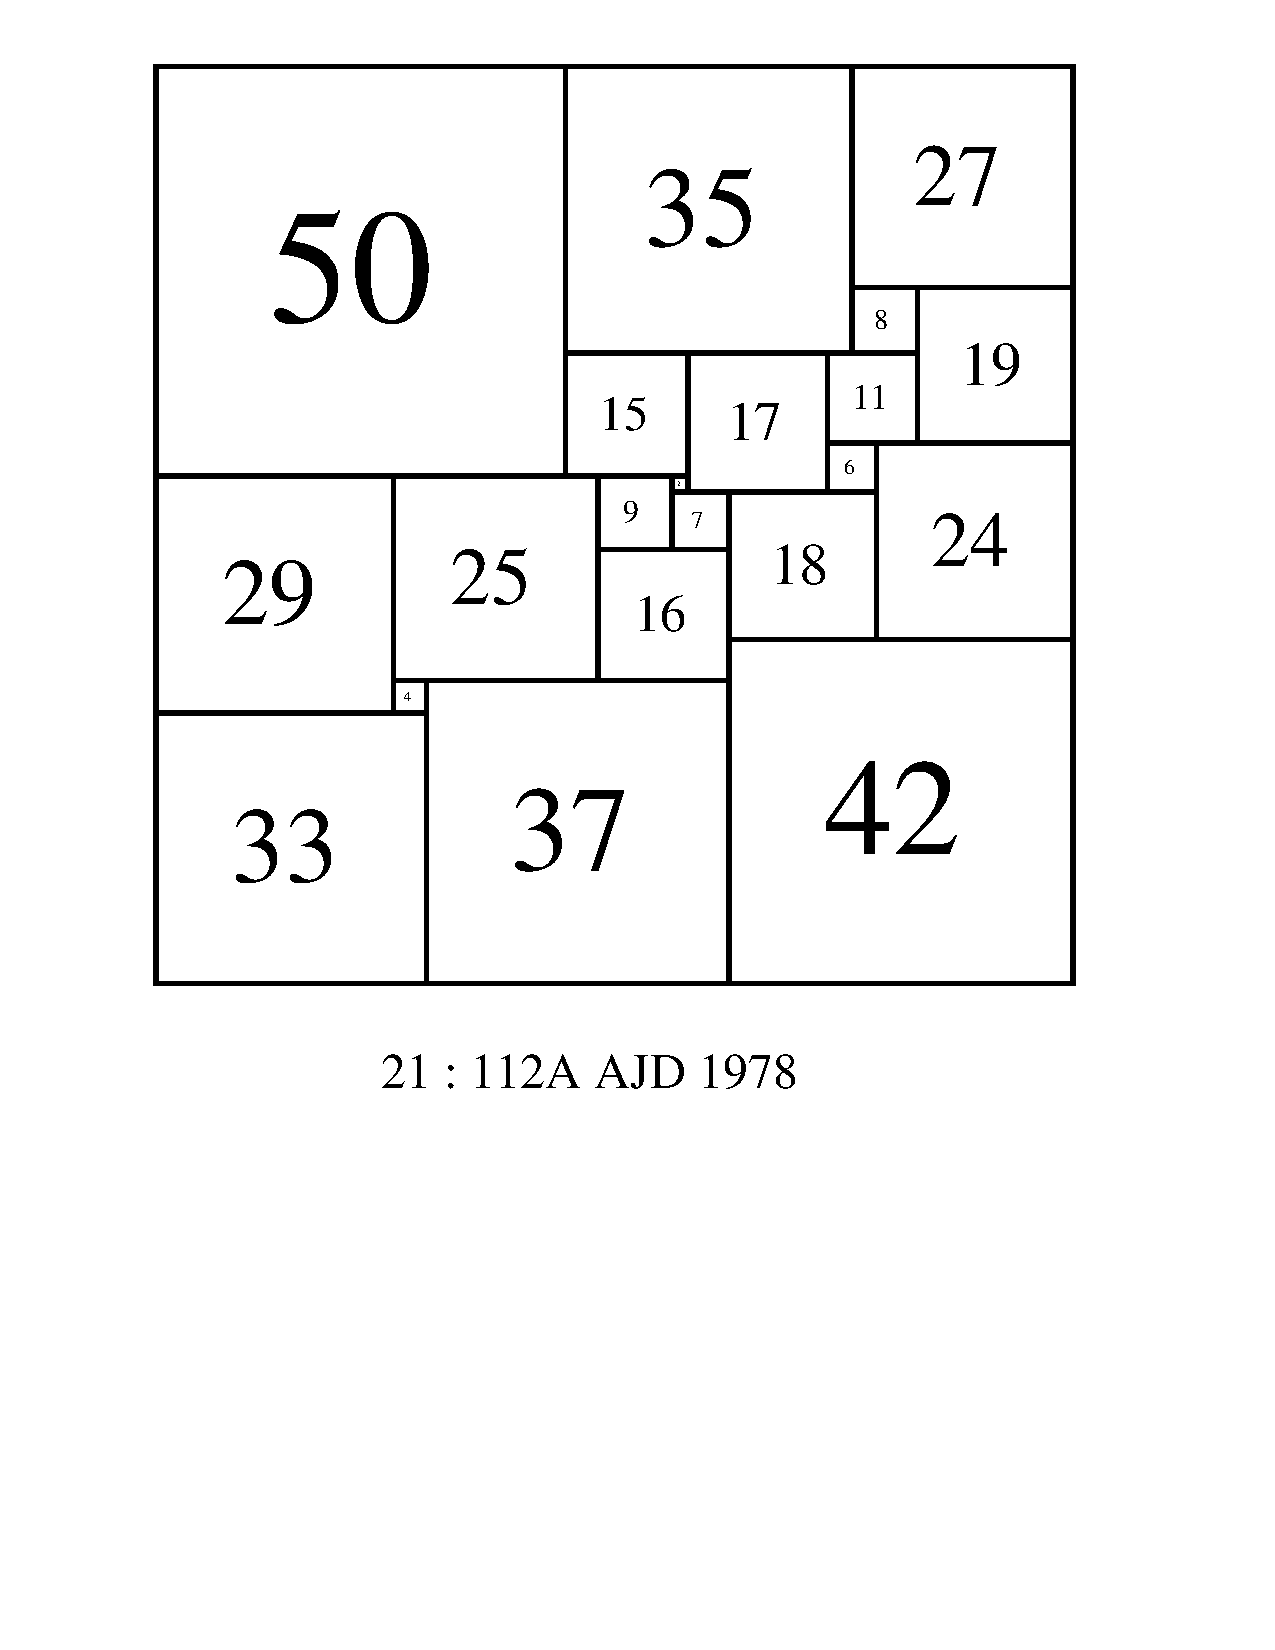
\includegraphics[width=6cm]{spsso21}
\end{frame}


\begin{frame}[fragile]
  \frametitle{Data}
  \begin{semiverbatim}
S = 1..21;
size =  [2,4,6,7,8,9,11,15,16,17,
         18,19,24,25,27,29,33,35,37,42,50];
box = 112;
  \end{semiverbatim}
\end{frame}

\begin{frame}[fragile]
  \frametitle{Square Packing Program (I)}
  \begin{semiverbatim}
include "globals.mzn";
set of int: S;
array[S] of int:size;
int: box;
include "squares.dzn";

array[S] of var 0..box:x;
array[S] of var 0..box:y;
  \end{semiverbatim}
\end{frame}

\begin{frame}[fragile]
  \frametitle{Square Packing Program (II)}
  \begin{semiverbatim}
constraint forall (i in S)
    (x[i]+size[i]<=box);
constraint forall (i in S)
    (y[i]+size[i]<=box);
constraint diffn(x,y,size,size);
constraint cumulative(x,size,size,box);
constraint cumulative(y,size,size,box);

solve satisfy;
  \end{semiverbatim}
\end{frame}

\begin{frame}[fragile]
  \frametitle{Solved with Chuffed}
  \begin{semiverbatim}
Running squares.mzn
x = array1d(1..21, [60, 33, 60, 53, 77, 53, 66, 62,
  37, 60, 42, 66, 42, 37, 85, 33, 0, 77, 0, 0, 62]);
y = array1d(1..21, [47, 79, 24, 42, 19, 49, 19, 47,
  42, 30, 24, 0, 0, 58, 0, 83, 79, 27, 42, 0, 62]);
----------
Finished in 4s 364msec

  \end{semiverbatim}
\end{frame}



\begin{frame}
  \frametitle{Job Shop Scheduling}
  \begin{itemize}
  \item Schedule a number of jobs
  \item Each job consists of a number of tasks
  \item Each task has a duration and must run on one specific machine
  \item Tasks of a job must be executed in sequence
    \item A machine can only work on one task as a time
  \end{itemize}
\end{frame}

\begin{frame}
  \frametitle{History}
  \begin{itemize}
  \item 10x10 instance proposed by Fisher\& Thompson
  \item Also known as 10x10 Muth \& Thompson instance (1963)
    \item Stayed as open problem for 25 years
  \item Solved by Carlier and Pinson in 1989   
  \end{itemize}
\end{frame}


\begin{frame}[fragile]
  \frametitle{Job Shop Data (I)}
  \begin{semiverbatim}
nrJobs= 6;
nrRes= 6;
taskUse= [|
   2, 0, 1, 3, 5, 4|
   1, 2, 4, 5, 0, 3|
   2, 3, 5, 0, 1, 4|
   1, 0, 2, 3, 4, 5|
   2, 1, 4, 5, 0, 3|
   1, 3, 5, 0, 4, 2 |];
taskDuration= [|
   1, 3, 6, 7, 3, 6|
   8, 5, 10, 10, 10, 4|
   5, 4, 8, 9, 1, 7|
   5, 5, 5, 3, 8, 9|
   9, 3, 5, 4,3, 1|
   3, 3, 9, 10, 4, 1 |];
  \end{semiverbatim}
\end{frame}

\begin{frame}[fragile]
  \frametitle{Job Shop Data (II)}
    \begin{semiverbatim}
nrJobs= 10;
nrRes= 10;

taskUse= [|
	0, 1, 2, 3, 4, 5, 6, 7, 8, 9|
	0, 2, 4, 9, 3, 1, 6, 5, 7, 8|
	1, 0, 3, 2, 8, 5, 7, 6, 9, 4|
	1, 2, 0, 4, 6, 8, 7, 3, 9, 5|
	2, 0, 1, 5, 3, 4, 8, 7, 9, 6|
	2, 1, 5, 3, 8, 9, 0, 6, 4, 7|
	1, 0, 3, 2, 6, 5, 9, 8, 7, 4|
	2, 0, 1, 5, 4, 6, 8, 9, 7, 3|
	0, 1, 3, 5, 2, 9, 6, 7, 4, 8|
	1, 0, 2, 6, 8, 9, 5, 3, 4, 7 |];
    \end{semiverbatim}
\end{frame}

\begin{frame}[fragile]
  \frametitle{Job Shop Data (III)}
    \begin{semiverbatim}
taskDuration= [|
	29, 78,  9, 36, 49, 11, 62, 56, 44, 21|
	43, 90, 75, 11, 69, 28, 46, 46, 72, 30|
	91, 85, 39, 74, 90, 10, 12, 89, 45, 33|
	81, 95, 71, 99,  9, 52, 85, 98, 22, 43|
	14,  6, 22, 61, 26, 69, 21, 49, 72, 53|
	84,  2, 52, 95, 48, 72, 47, 65,  6, 25|
	46, 37, 61, 13, 32, 21, 32, 89, 30, 55|
	31, 86, 46, 74, 32, 88, 19, 48, 36, 79|
	76, 69, 76, 51, 85, 11, 40, 89, 26, 74|
	85, 13, 61,  7, 64, 76, 47, 52, 90, 45 |];
    \end{semiverbatim}
\end{frame}

\begin{frame}
  \frametitle{Example Solution}
  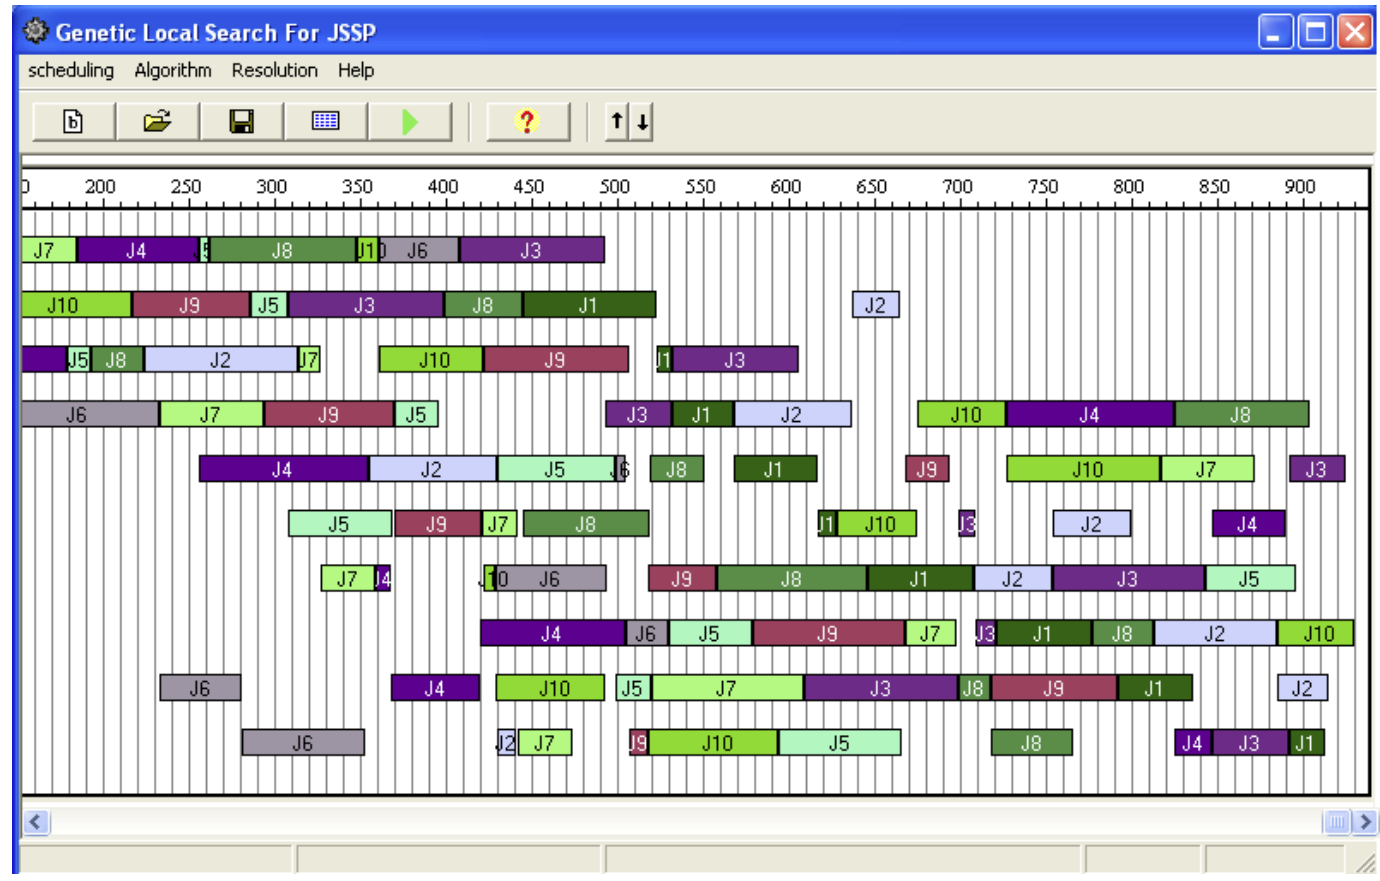
\includegraphics[width=10cm]{ft10}
  {\scriptsize screenshot from:
  A LOCAL SEARCH GENETIC ALGORITHM FOR THE JOB SHOP SCHEDULING PROBLEM
Kebabla Mebarek, Mouss Leila Hayat and Mouss Nadia}
\end{frame}


\begin{frame}[fragile]
  \frametitle{Job-Shop Program (I)}
  \begin{semiverbatim}
include "globals.mzn";
int:nrJobs;
int:nrRes;

set of int: J=1..nrJobs;
set of int: R=1..nrRes;

array[J,R] of int:taskUse;
array[J,R] of int:taskDuration;
include "mt06.dzn";
int:ub =sum(j in J,r in R)(taskDuration[j,r]);

array[J,R] of var 0..ub:start;
var 0..ub:objective;
  \end{semiverbatim}
\end{frame}

\begin{frame}[fragile]
  \frametitle{Job-Shop Program (II)}
  \begin{semiverbatim}
constraint forall(j in J) 
    (objective >= start[j,nrRes]+
                  taskDuration[j,nrRes]);
constraint forall(j in J, r in 1..nrRes-1)
    (start[j,r+1] >= start[j,r]+
                     taskDuration[j,r]);
constraint forall (r in R)
(cumulative(
  [start[j,k]|j in J, k in R
    where taskUse[j,k]+1=r],
  [taskDuration[j,k]|j in J, k in R
    where taskUse[j,k]+1=r],
  [1|j in J, k in R
    where taskUse[j,k]+1=r],
  1)
);
  \end{semiverbatim}
\end{frame}

\begin{frame}[fragile]
  \frametitle{Job-Shop Program (III)}
  \begin{semiverbatim}
solve minimize objective;
  \end{semiverbatim}
\end{frame}





